\section{方法}

\subsection{总体思路}

本文方法建立在统一的层级 H3 区域预测框架上。输入端，历史轨迹被编码为区域 token、父层区域 token、数值运动特征、mask 特征和轻量上下文；输出端，所有模型共享 coarse-to-fine H3 输出头，先预测父层区域，再在父层条件下预测子区域分布。这样可以把研究重点放在时间证据如何被读取和融合上，而不是把收益混入不同输出空间或评价口径。

Horizon-Router 的核心思路是把“不同提前量需要不同历史证据”显式写进模型。模型首先用多尺度 horizon-query 编码器为每个预测时域读取细尺度和粗尺度历史证据；随后用三个 expert 表达不同时间尺度的运动信息，并由 horizon-level router 生成时域相关的融合权重。推理阶段，融合后的特征进入共享层级 H3 输出头，得到每个 horizon 上的细粒度区域概率。

\begin{figure}[!t]
\centering
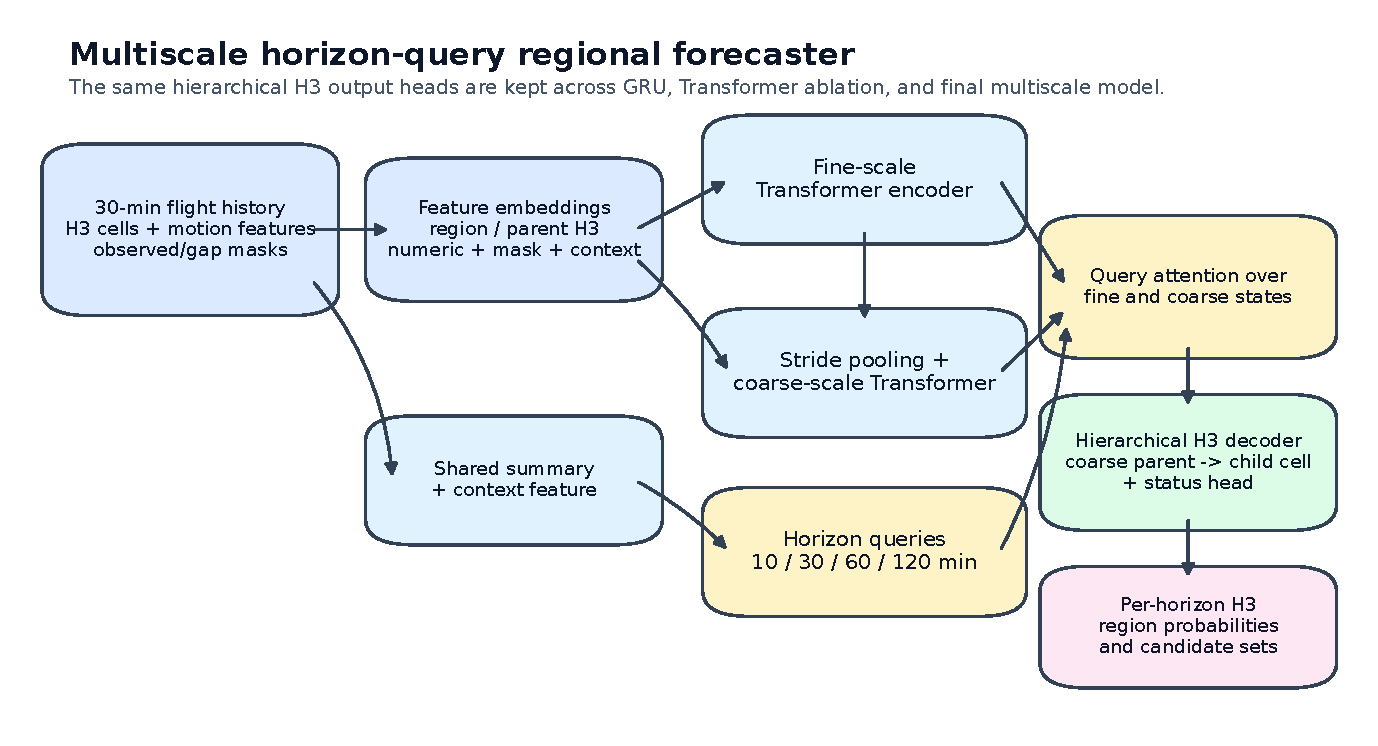
\includegraphics[width=\textwidth]{figures/fig1_method_architecture.pdf}
\caption{Horizon-Router 方法总览。历史轨迹和轻量上下文首先被编码为 H3/父层 token 与数值特征；多尺度 horizon-query 编码器为每个预测时域检索细尺度和粗尺度历史证据；global、coarse-stable 和 local-causal 三个 expert 经 horizon-level router 融合后，进入 coarse、status 和 child heads，输出层级 H3 区域概率。}
\label{fig:method-architecture-zh}
\end{figure}

\subsection{输入表示与层级 H3 输出}

对每个历史时间步 $z_t=(r_t,p_t,u_t,m_t)$，模型分别学习输入区域 embedding、父层区域 embedding，并将数值特征和 mask 特征线性投影到同一隐空间：
\begin{equation}
\tilde{z}_t = [E_r(r_t); E_p(p_t); W_u u_t; W_m m_t].
\end{equation}
其中 $r_t$ 是输入分辨率 H3 cell，$p_t$ 是其父层 cell，$u_t$ 包含位置、位移、高度、速度、航向、时间间隔等数值特征，$m_t$ 包含 \texttt{observed\_flag} 与 \texttt{gap\_flag}。模型根据观测标记、缺口标记和 unknown token 构造时间有效掩码；该掩码被 Transformer attention、池化和局部编码模块共享，用于抑制填充片段和缺口补齐片段的影响。样本级上下文 $c$ 经过单独线性层投影后参与后续编码。

对每个预测时域 $h_j$，层级输出头预测粗区域、状态和条件子区域：
\begin{equation}
p(y_j^{(c)}, y_j^{(f)}, s_j \mid X,c,h_j)
=
p(s_j \mid X,c,h_j)
p(y_j^{(c)} \mid X,c,h_j)
p(y_j^{(f)} \mid y_j^{(c)},X,c,h_j).
\end{equation}
训练时，子区域交叉熵使用真值粗区域标签作为条件，以稳定学习父子层级对应关系。推理时，模型从粗区域分布中选取 top-$K_j$ 个父区域，再计算每个父区域下的条件子分布，并将父层概率质量散射到细粒度 H3 cell。本文完整实验中使用的父层 top-$K$ 为 $[64,48,48,12]$。

\subsection{多尺度 Horizon-Query 编码器}

单一历史摘要难以同时服务 10 分钟和 120 分钟预测。本文先用带有效掩码的 Transformer encoder 得到细尺度历史序列
\begin{equation}
H^{(f)}=\mathrm{Enc}(W_z\tilde{Z}+P),
\end{equation}
并通过 masked mean pooling 与上下文投影拼接为共享基特征 $b$。随后，模型按 stride $=2$ 对 $H^{(f)}$ 做带掩码的局部均值池化，再经一个粗尺度 Transformer encoder 得到
\begin{equation}
H^{(c)} = \mathrm{Enc}_{c}(\mathrm{Pool}(H^{(f)})).
\end{equation}

对每个 horizon，模型维护可学习 horizon embedding $e_j$，并构造时域查询向量
\begin{equation}
q_j = W_q[b;e_j].
\end{equation}
该查询分别对细尺度序列和粗尺度序列做交叉注意力：
\begin{equation}
\alpha_j^{(f)}=\mathrm{softmax}(q_j {H^{(f)}}^\top),\qquad
\alpha_j^{(c)}=\mathrm{softmax}(q_j {H^{(c)}}^\top),
\end{equation}
\begin{equation}
z_j^{(f)}=\alpha_j^{(f)}H^{(f)},\qquad
z_j^{(c)}=\alpha_j^{(c)}H^{(c)}.
\end{equation}
多尺度 horizon-query 特征写为
\begin{equation}
g_j=\phi_g([b;z_j^{(f)};z_j^{(c)};e_j]).
\end{equation}
这里的 $g_j$ 同时也是 Horizon-Router 中的 global expert：它保留完整历史、细尺度注意力和粗尺度注意力，是 warm-start 时最强的单路径预测分支。

\subsection{Horizon-Router 三专家融合}

Horizon-Router 在 global expert 之外加入两个分工明确的 expert。coarse-stable expert 只依赖粗尺度序列摘要和粗尺度注意力：
\begin{equation}
c_j=\phi_c([b^{(c)};z_j^{(c)};e_j]),
\end{equation}
其中 $b^{(c)}$ 是粗尺度序列的 masked mean pooling 与上下文投影拼接。该分支强调阶段性趋势和粗粒度稳定演化，主要服务中长时域预测。

local-causal expert 只读取最近若干历史步，并使用因果 Transformer encoder 抑制对未来位置的泄漏。设最近局部序列为 $H^{(\ell)}$，则短时 horizon 的局部特征为
\begin{equation}
\ell_j=\phi_\ell([b;z_j^{(\ell)};e_j]),\qquad
z_j^{(\ell)}=\mathrm{Attn}(q_j,H^{(\ell)}).
\end{equation}
在实现中，local-causal expert 只对预设的短时 horizon 激活；对更长 horizon，该分支通过 active expert mask 被置为不可用。这个边界很重要：局部机动对 10 或 30 分钟预测有价值，但不应被强行解释为 120 分钟区域需求的主证据。

router 在每个 horizon 上读取三个 expert 特征和 horizon embedding，输出融合权重：
\begin{equation}
w_j=\mathrm{softmax}(R([g_j;c_j;\ell_j;e_j]))\in\mathbb{R}^3.
\end{equation}
最终解码特征为
\begin{equation}
d_j=w_{j,g}g_j+w_{j,c}c_j+w_{j,\ell}\ell_j.
\end{equation}
$d_j$ 被送入共享的粗区域头、状态头和条件子区域头。与简单加深单一路径编码器相比，这一结构让模型可以在时域层面选择历史证据来源，而不必要求所有 horizon 使用同一种时间摘要。

\subsection{训练目标与路由约束}

基础层级损失由粗区域、子区域和状态交叉熵组成。设 $\mathcal{V}$ 为 batch 中有效 horizon 集合，则
\begin{equation}
\mathcal{L}_{\text{hier}}
=
\frac{1}{|\mathcal{V}|}
\sum_{j\in\mathcal{V}}
\left(
\mathcal{L}^{(j)}_{\text{coarse}}
+
\mathcal{L}^{(j)}_{\text{child}}
+
\mathcal{L}^{(j)}_{\text{status}}
\right).
\end{equation}

为了避免 router 过早偏向单一 expert，本文加入 loss-aware router supervision。对每个有效 horizon 和每个 active expert，模型临时用该 expert 特征通过共享输出头计算 expert loss $L_{j,e}$，并构造 soft target：
\begin{equation}
\hat{w}_{j,e}=
\frac{\exp(-L_{j,e}/\tau)}
{\sum_{e'\in\mathcal{A}_j}\exp(-L_{j,e'}/\tau)}.
\end{equation}
其中 $\mathcal{A}_j$ 是 horizon $j$ 上的 active expert 集合，$\tau$ 是 router supervision temperature。router supervision 最小化 $\hat{w}_j$ 与 $w_j$ 之间的 KL 散度。active expert mask 用于屏蔽长时域上的 local-causal expert，避免该分支在不适用的 horizon 上接受错误激励。

本文还加入两个轻量约束。load balancing loss 将 router 权重拉向 active expert 上的均匀分布，防止单个 expert 长期占用全部概率质量；expert auxiliary loss 对 coarse-stable 和可用的 local-causal 分支施加输出头辅助监督，使这些分支即便未被 router 频繁选择也能保持可训练。global expert 通过主输出路径接受监督。

最后，模型使用 horizon-wise teacher distillation 稳定概率输出。训练时，从若干与层级输出兼容的强神经专家中按 horizon 构造混合教师分布，并对学生模型的 coarse、child 和 status 概率施加 KL 蒸馏项。总目标可写为
\begin{equation}
\mathcal{L}
=
\mathcal{L}_{\text{hier}}
+
\lambda_{\text{route}}\mathcal{L}_{\text{route}}
+
\lambda_{\text{bal}}\mathcal{L}_{\text{bal}}
+
\lambda_{\text{aux}}\mathcal{L}_{\text{aux}}
+
\lambda_{\text{distill}}\mathcal{L}_{\text{distill}}.
\end{equation}
完整实验使用的权重为：$\lambda_{\text{distill}}=0.08$，状态蒸馏权重 $0.01$，$\lambda_{\text{route}}=0.08$，$\lambda_{\text{bal}}=0.02$，$\lambda_{\text{aux}}=0.05$，router supervision temperature 为 $0.7$。

\subsection{推理概率支撑}

推理阶段，模型先从粗区域分布中保留每个 horizon 的 top-$K_j$ 父区域，再在这些父区域下展开条件子区域概率，并将父层概率质量散射回细粒度 H3 cell。为避免将概率分配给明显超出运动学范围的区域，本文在所有模型上使用相同的可达性掩码。该掩码根据当前 H3 cell 中心到目标 cell 中心的球面距离构造；若某目标 cell 的距离超过
\begin{equation}
d_{\max}(h_j)
=
v_{\max}\cdot 1.852 \cdot \frac{h_j}{60}
+
\Delta,
\end{equation}
则其概率被置零并重新归一化。本文默认采用 $v_{\max}=750$ knots、$\Delta=250$ km。该步骤只作为统一推理约束，不参与训练，也不作为 Horizon-Router 的方法贡献。
